\documentclass[12pt]{beamer}

% INCLUDE GRAPHICS
\usepackage{graphicx}

% TABLES
\newcommand{\ra}[1]{\renewcommand{\arraystretch}{#1}} % spaces in tables
\usepackage{booktabs}   % Allows the use of \toprule, \midrule and \bottomrule in tables for horizontal lines

% FONTS
% PdfLatex
% \usepackage[T1]{fontenc}
% \usepackage{pgf}
% \logo{\pgfputat{\pgfxy(-1,-0.435)}{\pgfbox[center,base]{
\includegraphics[width=1.2cm,natwidth=610,natheight=642]{KUNATLogo.pdf}}}}

% FONTS
% xelatex
\usepackage{fontspec}
% \fontspec[Path=../fonts/,]{
%     UprightFont = *-regular,
%     ItalicFont = *-italic,
%     Boldfont = *-bold
% }

% NOTE
% Add fonts to ~/.fonts for this to work
% \setsansfont{TeX Gyre Heros}
% \setsansfont{TeX Gyre Heros Cn}
% \setsansfont{Liberation Sans}
\setsansfont{Muli}
% \setsansfont{Helvetica Neue}

% Monospaces font
\setmonofont{Monaco}

% Use serif for Math environments
\usefonttheme[onlymath]{serif}

% TODO Use mono fonts

% CODE
\usepackage{listings} % Code block (source code) \begin{lstlisting}
\lstset{
    language=Python,                        % Code langugage
    commentstyle=\color{gray},              % Comments font
    basicstyle=\scriptsize\ttfamily,             % Code font, Examples: \footnotesize, \ttfamily
    keywordstyle=\bfseries\color{blue},
    stringstyle=\color{orange},
    numbers=left,                           % Line nums position
    numberstyle=\tiny,                      % Line-numbers fonts
    stepnumber=1,                           % Step between two line-numbers
    numbersep=5pt,                          % How far are line-numbers from code
    numbers=none,
    frame=lines,                             % A frame around the code
    rulecolor=\color{gray},
    tabsize=4,                              % Default tab size
    captionpos=b,                           % Caption-position = bottom
    breaklines=true,                        % Automatic line breaking?
    breakatwhitespace=false,                % Automatic breaks only at whitespace?
    showspaces=false,                       % Dont make spaces visible
    showstringspaces=false,                 % Dont make spaces visible in strings
    showtabs=false,                         % Dont make tabls visible
    belowskip=5pt,
    morekeywords={range, xrange},
    backgroundcolor=\color{white}
    % emph={[2]root,base}
    % morekeywords={one,two,three,four,five,six,seven,eight,
}

\newcommand{\code}[1]{{\small\ttfamily #1}} % \code{inline code}

%
% COLORS
%
\definecolor{kugreen}{RGB}{50,93,61}

\definecolor{orange}{RGB}{255,127,0}
\definecolor{green}{RGB}{0,153,51}
\definecolor{blue}{RGB}{3,115,187}
\definecolor{red}{RGB}{221,17,68}
\definecolor{gray}{RGB}{55,55,55}
\definecolor{black}{RGB}{0,0,0}

\definecolor{offwhite}{RGB}{249,242,215}
\definecolor{foreground}{RGB}{23,23,23}
\definecolor{background}{RGB}{255,255,255}
\definecolor{subtitle}{RGB}{102,255,204}
\definecolor{hilight}{RGB}{102,255,204}
\definecolor{vhilight}{RGB}{255,111,207}
\definecolor{lolight}{RGB}{155,155,155}


%
% BEAMER STYLE COLORS
%
\setbeamercolor{titlelike}{fg=black}
\setbeamercolor{subtitle}{fg=blue}
\setbeamercolor{institute}{fg=gray}
\setbeamercolor{normal text}{fg=foreground,bg=background}
\setbeamercolor{item}{fg=foreground} % color of bullets
\setbeamercolor{subitem}{fg=gray}
\setbeamercolor{itemize/enumerate subbody}{fg=gray}

\setbeamerfont{itemize/enumerate subbody}{size=\footnotesize}
\setbeamerfont{itemize/enumerate subitem}{size=\footnotesize}

\setbeamerfont{footnote}{size=\tiny}

\setbeamersize{text margin left=10pt}
\setbeamersize{text margin right=10pt}
\setbeamersize{sidebar width right=0pt}
\setbeamersize{sidebar width left=0pt}

%
% REMOVES THE NAVIGATION BAR
%
\beamertemplatenavigationsymbolsempty


% BEAMER TEMPLATES


%
% BEAMER BACKGROUND
%
\usebackgroundtemplate{

    \rule{0pt}{0.97\paperheight}%
    \hspace*{1.15\paperwidth}%
    \makebox[0pt][r]{%
        
\includegraphics[width=100pt,natwidth=610,natheight=642]{KUNATLogo.pdf}
    }

}


%
% BEAMER HEADLINE
%
\setbeamertemplate{headline}{}


%
% BEAMER TITLE
%
\setbeamertemplate{frametitle}
{
    \begin{centering}
    \insertframetitle\par
    \end{centering}
}


%
% BEAMER FOOTER
%
\setbeamertemplate{footline}[text line]
{%
    \vbox{%
        \insertvrule{0.5pt}{kugreen}

        \vspace{2pt}

        \strut{
        % \rmfamily\itshape
        \expandafter\insertshorttitle
        \expandafter\insertauthor
        \insertshortinstitute
        }
        \hfill\strut{
        }
        \hfill\strut{
            \insertframenumber\,/\,\inserttotalframenumber
        }

        \vspace{1pt}
    }
}


%
% TITLE PAGE
%
% \setbeamertemplate{title page}
% {
%     % Remove beamer background
%     \setbeamertemplate{background}{}
% 
%     \begin{beamercolorbox}[center]{beamer color}
% 
%         {
%             \huge
%             \color{kugreen}
%             \inserttitle
%         }
%         \bigskip
%         \bigskip
% 
%         % 
\includegraphics[width=2cm]{KUNATLogo}
% 
%         \bigskip
%         {
%             \bf
%             \rmfamily
%             {\large \insertauthor}
%         }
% 
%         \smallskip
%         {
%             \rmfamily
%             \footnotesize
%             \insertinstitute
%         }
% 
%         {
%             \rmfamily
%             \footnotesize
%             \insertdate
%         }
% 
%     \end{beamercolorbox}
% 
%     % Do not count the title page
%     \addtocounter{framenumber}{-1}
% }


\usepackage{soul}

\title[]{Week 1\\Molecular Statistics}


\institute[, University of Copenhagen]{C315B\\ Department of Chemistry \\ University of Copenhagen}

\author[J. C. Kromann]{Jimmy Charnley Kromann}

\date{
    \code{\scriptsize help: jimmy@charnley.dk}
}




% ===============
% begin slides
% ===============


\begin{document}

{
\usebackgroundtemplate{}
\begin{frame}[plain]
    \titlepage
    \addtocounter{framenumber}{-1}
\end{frame}
}

{

\usebackgroundtemplate{

    \rule{0pt}{1.0\paperheight}%
    \hspace*{1.15\paperwidth}%
    \makebox[-8pt][r]{%
        
\includegraphics[width=250pt]{images/panic.png}%
    }

}

\begin{frame}[fragile]

    \frametitle{Motivation}

     Why, oh why. Do I really need to learn this?!

     \bigskip
     \bigskip
     \bigskip
     \bigskip
     \bigskip

     \begin{itemize}
         \item Bachelor project
         \item Master project
         \item PhD project
         \item Real life science
     \end{itemize}

\end{frame}
}

\begin{frame}[fragile]

    \frametitle{Motivation}

    \begin{columns}[t]

        \column{0.4\linewidth}

            \begin{itemize}
                \item Data processing
                \item Data analysis
                \item Simulations
                \item Plotting
            \end{itemize}

            \bigskip

            Python > All
            \begin{itemize}
                \item \st{Excel}
                \item \st{Matlab}
                \item \st{Gnuplot}
                \item \st{R}
            \end{itemize}

        \column{0.5\linewidth}

            \centering

            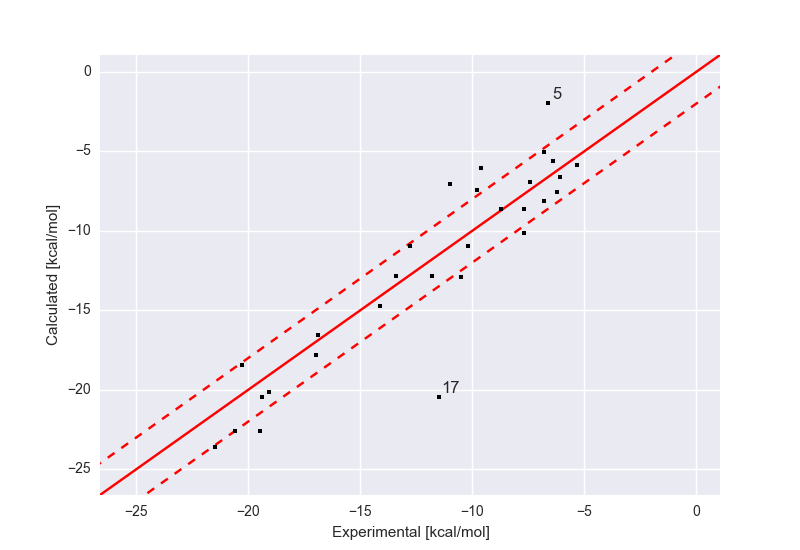
\includegraphics[width=0.8\textwidth]{images/plot1.png}

            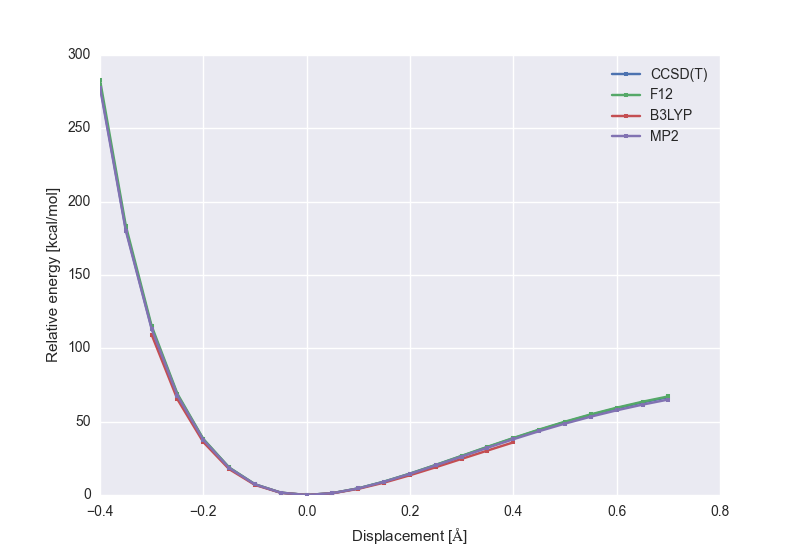
\includegraphics[width=0.8\textwidth]{images/plot2.png}

    \end{columns}

\end{frame}


\begin{frame}[fragile]

    \frametitle{Motivation}

    \begin{center}
        Video %TODO
    \end{center}

\end{frame}


\begin{frame}[fragile]

    \frametitle{Executing Python}

    \begin{columns}[t]

        \column{0.4\linewidth}

            \begin{center}
                python first\_program.py
            \end{center}

\begin{lstlisting}
print "Hello World"

for i in range(5):
    print 'i', i
\end{lstlisting}

        \column{0.4\linewidth}

            \begin{center}
                Output
            \end{center}

\begin{lstlisting}
Hello World
i 0
i 1
i 2
i 3
i 4
\end{lstlisting}


    \end{columns}


\end{frame}



\begin{frame}[fragile]

    \frametitle{Programming in Python}

    \begin{itemize}
        \item Variables and Datatypes
        \item Operators
        \item Comments
        \item Indentation
        \item Modules
        \item Looping
        \item If-else
    \end{itemize}

\end{frame}


\begin{frame}[fragile]

    \frametitle{Variables and Datatypes}

    \begin{columns}[t]

        \column{0.2\linewidth}

            \begin{itemize}
                \item String
                \item Integer
                \item Float
                \item List
            \end{itemize}

        \column{0.6\linewidth}

\begin{lstlisting}
name = "Peter"    # String
age = 31          # Integer
height = 1.80     # Float

s = [2, 4, 8, 16] # List
\end{lstlisting}

    \end{columns}

    \bigskip

    \centering

\begin{tabular}{llllllll}
   $i$  & 0  & 1 & 2 & 3 \\ \hline
$s(i)$ & 2 & 4 & 8 & 16  
\end{tabular}



\end{frame}



\begin{frame}[fragile]

    \frametitle{Operators}

    \begin{columns}[t]

        \column{0.5\linewidth}

% +linewidthAddition - Adds values on either side of the Operators a + b will give 30
% -30Subtraction - Subtracts right hand operand from left hand operand a - b will give -10
% *10Multiplication - Multiplies values on either side of the Operators a * b will give 200
% /200Division - Divides left hand operand by right hand operand b / a will give 2
% %giveModulus - Divides left hand operand by right hand operand and returns remainder b % a will give 0
% **giveExponent - Performs exponential (power) calculation on Operators a**b will give 10 to the power 20
 
        \begin{tabular}{l l}

            \bf Operator & \bf Description \\

            \midrule
            \code{+}  & Addition \\
            \code{-}  & Subtraction \\
            \code{*}  & Multiplication \\
            \code{/}  & Division \\
            \code{\%} & Modulus \\
            \code{**} & Exponent ($a^b$) \\
            \midrule

        \end{tabular}


        \column{0.4\linewidth}

\begin{lstlisting}
print 5.0 + 5.0
print 5.0 - 5.0
print 5.0 / 5.0
print 5.0 % 5.0
print 5.0**5.0

print 3 / 2
print 3.0 / 2.0

\end{lstlisting}

    \end{columns}

\end{frame}


\begin{frame} 
    \frametitle{15min break}
    \begin{center}
        
\includegraphics[width=0.65\textwidth]{images/barbie1.png}
    \end{center}
\end{frame}

\begin{frame}[fragile]

    \frametitle{Comments and Indentation}

    \begin{columns}[t]

        \column{0.5\linewidth}

            Python is indentation based

            Indentation is {\bf 4 spaces}

            \bigskip
            \bigskip

            Comments are very usefull when looking at previous code

        \column{0.4\linewidth}


\begin{lstlisting}
a = 5
 a = 5 # Error, why?

\end{lstlisting}

\begin{lstlisting}
# Line comment

"""
Multiline
comment
"""
\end{lstlisting}

    \end{columns}

\end{frame}




\begin{frame}[fragile]

    \frametitle{Looping}


\begin{lstlisting}
my_list = [2.0, 4.0, 8.0]

for x in my_list:
    print x
\end{lstlisting}


\begin{lstlisting}
for i in range(24):
    print 'i', i
\end{lstlisting}


\begin{lstlisting}
x_list = [i**2 for i in range(10)]
\end{lstlisting}


\end{frame}


\begin{frame}[fragile]

    \frametitle{Modules}

Always in the top of the program

Use Python modules or local \code{.py}-files

\bigskip

\begin{lstlisting}
import random
import matplotlib.pyplot as plt
\end{lstlisting}

\begin{lstlisting}
import video  # imports video.py
\end{lstlisting}


\end{frame}



\begin{frame}[fragile]

    \frametitle{Looping and Double Looping}

    \begin{center}
        15 min
    \end{center}

    \begin{columns}[t]

        \column{0.5\linewidth}

            \begin{align*}
                K = \sum_{j=1}^{50} j^2
            \end{align*}


        \column{0.5\linewidth}

            \begin{align*}
                K = \sum_{i=5}^{10} \sum_{j=1}^{42} i \cdot j^{1/2}
            \end{align*}


    \end{columns}

    \bigskip
    \bigskip

\end{frame}

\begin{frame}[fragile]

    \frametitle{Looping and Double Looping}

    \begin{columns}[t]

        \column{0.5\linewidth}

            \begin{align*}
                K = \sum_{j=1}^{50} j^2
            \end{align*}

\begin{lstlisting}
j_list = range(1, 51)
k = 0

for j in j_list:
    k = k + j**2 

print k
\end{lstlisting}


        \column{0.5\linewidth}

            \begin{align*}
                K = \sum_{i=5}^{10} \sum_{j=1}^{42} i \cdot j^{1/2}
            \end{align*}
\scriptsize
\begin{lstlisting}
j_list = range(1, 42)
i_list = range(5, 10)
k = 0

for i in i_list:
    for j in j_list:
        k = k + i * j**(1.0/2.0)

print k
\end{lstlisting}


    \end{columns}



\end{frame}


\begin{frame}[fragile]

    \frametitle{If and Else}

    \centering

    \begin{tabular}{l l}

        \bf Operator & \bf Meaning \\

        \midrule

        \code{<}  & Is less than \\
        \code{<=} & Is less than or equal to \\
        \code{>}  & Is greater than \\
        \code{>=} & Is greater than or equal to \\
        \code{==} & Is equal to \\
        \code{!=} & Is not equal to\\

    \end{tabular}

    \bigskip

\begin{lstlisting}
k = 1.0

if k == 5.0:
    print "The number is five"

if k < 5.0:
    print "Smaller than five"

\end{lstlisting}


\end{frame}






\begin{frame}[fragile]

    \frametitle{First Exercise}

\begin{lstlisting}
import random
import matplotlib.pyplot as plt

# initialize some variables
n_particles = 100
box_width = 10.0
n_steps = 1
dt = 0.01

# create the x- and y-coordinates
pos_x = [random.random() for i in range(n_particles)]
pos_y = [random.random() for i in range(n_particles)]

# plot the x- and y-coordinates in a figure.
plt.plot(pos_x, pos_y, 'ro')
plt.axis((-box_width, box_width, -box_width, box_width))
plt.savefig('coordinates_start.png')

\end{lstlisting}


\end{frame}




% LAST FRAME

\frame
{
    \frametitle{The End}

    \bigskip
    jimmy@charnley.dk

    \bigskip

    C315B

}




%%%%%%%%%%%%%%%%%%%%%%%%%%%%%%%%%%%%%%%%%%%%%%%%%%%%%%%%%%%%%%%%%%%%%%
%% END FRAMES
%%%%%%%%%%%%%%%%%%%%%%%%%%%%%%%%%%%%%%%%%%%%%%%%%%%%%%%%%%%%%%%%%%%%%%

\end{document}

